\section{Method}
\label{sec:method}

\subsection{Dataset}
The dataset consists of the set of videos of the
English-language version of {\it Peppa Pig}. In addition to the raw
videos we  also use the annotation created by
\citet{papasarantopoulos2021narration}.

These annotations feature written transcriptions aligned with the
audio as well as segmentation into {\it dialog} and {\it
  narration}.\footnote{It should be noted that the quality of the
  alignment and segmentation in the original dataset is variable. In
  cases where exact alignment is needed, such as for word-level
  analyses, we re-align the transcriptions using
  \url{github.com/lowerquality/gentle}.}  Dialogs are the parts spoken
by the characters, while narrations are comments inserted by the
narrator, which are more descriptive in nature. All the narration
segments are uttered by the same actor. We use the dialogs for
training the model, and set aside the narrations for evaluation
purposes only. A small portion of the dialog data is also used for
evaluation.

Specifically, we use dialog from episodes 1--196 for training, and
197--209 for validation. We set aside narrations from episodes 1--104
for validation and 105--209 for testing.


\subsection{Preprocessing}
For training, we do not use word or sentence level segmentation in
order to make the setting more naturalistic. Instead we split the
dialog sections into {\bf XXX}  second non-overlapping fragments. The video
is subsampled to 10 frames per second, and to $180\times 100$ resolution. The
audio is converted to mono by averaging the two channels  and the raw
waveform is used as input.


For evaluation we have a number of different conditions and evaluation
metrics described in detail in \Cref{sec:eval} and in some of these
conditions we use the subtitles to guide
segmentation. \Cref{tab:ds-stat} shows the basic statistics of the
training and validation splits.

\begin{table}
  \centering
  \begin{tabular}{llrr}
	\toprule
	Split &      Type &  Size (h) &  \# Clips \\
	\midrule
	train &    dialog &     10.01 &    15666 \\
	val &    dialog &      0.66 &     1026 \\
	val & narration &      0.94 &     1467 \\
	test & narration &      0.64 &     1006 \\
	\bottomrule
\end{tabular}

  \caption{Dataset statistics. For the triplet condition, videos are
    split such that each segment corresponds to a line of
    subtitles. For the non-triplet condition, videos are split into
    3.2s segments.}
  \label{tab:ds-stat}
\end{table}


\subsection{Evaluation}
\label{sec:eval}
The most common approach to evaluation for visually grounded models
trained on spoken image captions is caption-to-image retrieval (often
combined with image-to-caption retrieval): in fact this technique is
has been carried over from text-based image-caption modeling
\citet{chrupala-visually-2021}.
 With the
standard spoken caption dataset this approach is unproblematic since
the content of the captions is not correlated with extra-linguistic
clues in the speech signal, such as speaker identity (since speakers
are randomly assigned to captions) or non-speech environmental
noise. Thus in this setting, a retrieval metric measures the ability of the
model to match spoken utterances to images based on their semantic
content. This not the case for the {\it Peppa Pig} dataset: here we
can expect that when a video segment depics a particular character
(e.g.\ George) then the audio in this segment is more likely to contain
utterances spoken by the voice actor playing George. George has a
favorite toy dinosaur: when this toy appears in a video segment we can
likewise expect higher than random chance of George's voice in the
audio. Due to these factors, in a naive retrieval setting, a model
could obtain a high score by mostly capturing these non-linguistic
correlations.

In order to (partially) alleviate these concerns we leverage the
narrator speech in the videos. These utterances are always spoken by
the same actor, so speaker identity cannot be used as a clue for
matching video and audio. Furthermore, the narration segments are akin
to video captions in that they tend to describe what is happening in
the video and thus their semantic content is more strongly
correlated with the content of the video than in the case of the
dialog, which is also a desirable feature for the purposes of system
evaluation.

\paragraph{Retrieval}
For the retrieval evaluation, as for training, we use fixed
segmentation into XXXXXXXs clips. We encode each audio clip in the
validation (or test) data using the speech encoder part of the model;
we encode each video clip using the video encoder. We then measure
cosine similarity between the audio clip and all the video clips. If
the video clip corresponding to the audio is among the $n$ most
similar video clips, we count that as a success. The proportion of
successes across all audio clips gives us the retrieval metric known
as recall@$n$: specifically in this paper we focus on $n=10$.
\todo{GC: Add fixed vs jitter condition for retrieval too.} 
\paragraph{Triplets}
Retrieval metrics such as recall@10 have some disadvantages. Firstly
the absolute value of this metric is hard to interpret as it depends
crucially on the size of the candidate set (e.g.\ the size of the
validation/test set). Thus these numbers cannot be directly between
different datasets. Secondly, if
we wanted to compare model performance with human performance, we
could not feasibly ask human participants to provide the quadratic
number of audio-video similarity judgments needed. For these reasons
we evaluate model performance using the following simplified,
controlled scenario: We extract clips aligned to a single subtitle
line, group them by length, and for each pair of same-length video
clips\footnote{To keep test items independent, the pairing of video
  clips is done such that each clip only occurs as a member of a single
  triplet.}, we extract the audio from one of them (selected at
random) -- this is our {\it anchor}. The video clip from which the
anchor was taken is the {\it positive} one, which the other video clip
is the {\it negative} one. This triplet of stimuli form a single test
item.  We use the model's audio encoder to encode the anchor, and the
video encoder to encode both video clips. We then check whether anchor
is more similar to the positive or negative clips in terms of cosine
similarity.  More precisely, {\it triplet accuracy} is the mean over
all triplets of the following quantity:
\begin{equation}
  \frac{\mathrm{signum}(\mathrm{cosine}(A, P) - \mathrm{cosine}(A, N)) + 1}{2}
  \label{eq:triplet-acc}
\end{equation}
with $A$ being the anchor, $P$ positive and $N$ negative. The triplet
accracy metric is inspired by the ABX score of \citet{schatz2016abx}.
For triplet accuracy, regardless of the specific set of test items, we
expect random-guessing performance to be at 0.5, and perfect
performance to be 1.0.  To improve the reliability of this metric and
provide information on its variance, triplets can be resampled $N$
times from the dataset, and the mean accuracy and spread around the mean
reported.

\paragraph{Targeted Triplets}
Inspired by 2-alternative forced choice (2AFC) paradigms in child
language acquisition \citep{noble2011comprehension, bergelson20126},
we design test trials that test the model's acquisition of grounded
semantics under controlled circumstances.

The test can be seen as a special case of the triplets evaluation as
described in the previous paragraph. Here, we aim to assess the
model's acquisition of the semantics of commonly occurring
words. Therefore, the \textit{targeted} approach considers, in
contrast to the general triplets evaluation, always pairs of triplets
with \textit{minimal differences} regarding one word in the
transcripts of the anchor audios (e.g., ``Peppa loves jumping'' and
``George loves jumping'' can be used to test whether the model can
discriminate the target word ``Peppa'' from the distractor word
``George'').


We search the transcripts of the validation data for phrases with
minimal differences with respect to the most commonly occurring nouns
and verbs.\footnote{There were not enough adjectives in the dataset
  perform a comprehensive analysis of their acquisition.} Details on
this search procedure can be found in Appendix
\ref{app:targeted_triplets_eval}. Based on each pair of phrases, we
create two counter-balanced test trials, an example and a
corresponding counter-example as depicted in
\Cref{fig:targeted_triplets}. Here, the anchor $A_x$ of the example
triplet is the audio of ``Peppa loves jumping'' ($a_p$), the positive
video $P_x$ is the corresponding video ($v_p$) and the negative video
$N_x$ is the video corresponding to ``George loves jumping'' ($v_g$):
$(A_x, P_x, N_x) = (a_p, v_p, v_g)$.  In the counter-example triplet,
the anchor $A_y$ is the audio of ``George loves jumping'', and the
positive and negative video are flipped:
$(A_y, P_y, N_y) = (a_g, v_g, v_p)$. In this way, we control the
evaluation for linguistic biases in the dataset and ensure that a
single-modality model that only considers the audio performs at chance
\citep{nikolaus-fourtassi-2021-evaluating}.

\begin{figure}
  \centering
  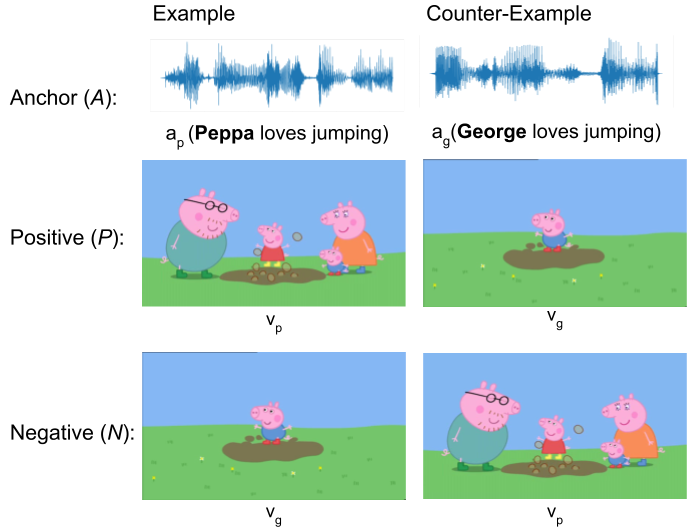
\includegraphics[width=.7\linewidth]{peppa_targeted_triplets.png}
  \caption{Targeted Triplets Evaluation}
  \label{fig:targeted_triplets}
\end{figure}

We measure overall targetet triplet accuracy using
\Cref{eq:triplet-acc}. Additionally, we report per-word accuracy by
calculating the triplet accuracy for all triplets that contain a given
word (e.g. ``Peppa'') either as target or distractor word, i.e. cases
in which the model needs to succeed in either choosing a video
containing the given word (the example triplet in Figure
\ref{fig:targeted_triplets}) or rejecting a video containing the given
word (the counter-example triplet in Figure
\ref{fig:targeted_triplets}).\footnote{Both the example and the
  counter-example shown in Figure \ref{fig:targeted_triplets} are also
  used to assess the acquisition of the word ``George''.}  We report
accuracy for all words for which we found at least 100 triplets.

\paragraph{Analysis of representations}
In addition to evaluating the model via task performance metrics, we
analyze the spoken utterance embeddings. There are a variety of
methods typically applied to this task, such as variants of diagnostic
probing, and representational similarity analysis (RSA). We focus on
a generalization of the latter approach.
The classical RSA was developed to analyze brain imaging data
\citep{kriegeskorte2008representational} and adapted for probing
neural network representations
\citep[e.g.][]{chrupala-alishahi-2019-correlating}. The method
consists in computing pairwise similarity scores for stimuli (such as
utterances) in two representation spaces: one being the subject of
analysis (i.e.\ neural activation space) and the other the benchmark
representation space (e.g.\ syntax tree space). The strength of
correlation between the pairwise similarity scores in the two spaces
quantifies to what extent the benchmark representation is encoded in
the neural activation patterns. In the current work we generalize this
idea such that it becomes possible to relate
neural activation similarity space and several different factors that
we hypothesize may be associated with it. Namely, we treat the
similarity scores in the neural activation space as regression targets
and fit a linear model with a number of predictors which 
correspond to control variables or hypothesized relevant factors.

Specifically, we compute pairwise cosine similarities between
model-embedded one-word or multi-word utterances from our validation data: these are
the regression targets. The variables are listed in \Cref{tab:grsa-variables}.

\begin{table}
  \centering
  \begin{tabular}{lp{0.7\linewidth}}\toprule
    Name              & Meaning \\\midrule
    sim$_2$           & Cosine similarity between representations,
                        from fully trained model,
                        of two audio clips \\
    sim$_1$           & Cosine similarity between representations,
                        from pre-trained-only model,  of two audio
                        clips \\
    semsim            & Cosine similarity between summed GloVe word-type-embeddings for two clips\\
    sametype          & Two clips correspond with the same transcription \\
    samespeaker       & Two clips uttered by same speaker\\
    sameepisode       & Two clips are from the same episode\\
    durationdiff      & Absolute difference in duration between two
                        clips\\
    durationsum       & Sum of the duration of the two clips\\
  \end{tabular}
  \caption{Variable definitions for the multiple RSA analysis.}
  \label{tab:grsa-variables}
\end{table}

\todo{THIS IS NOT QUITE RIGHT: For this analysis, we exclude word pairs where either word is out of
vocabulary for the GloVe dataset.} In order to obtain model embeddings
for the utterances, we use forced-alignment of audio with
corresponding subtitles, discarding cases where alignment fails.
%For
%the dialog condition the number of pairwise scores for the remaining
%tokens is X; for the narration condition it is Y.

The coefficients of the regression model serve as the estimates of the
strength of the association of each predictor with the target variable
(pairwise similarity), while controlling for the other predictors. 


\subsection{Model}

We adapt the high-level modeling approach from work on spoken
image-caption data
\citep{harwath2016unsupervised,chrupala-etal-2017-representations}:
our objective function is based on a triplet-loss with margin which
encourages the matching audio and video clip to be projected nearby in
the embedding space, and mis-matching audio and video clips to be far
away:
\begin{equation}
  \ell = \sum_{av}\left[\sum_{a'} \max(0, S_{a'v} - S_{av} +
    \alpha) + \sum_{v'} \max(0, S_{av'} - S_{av} + \alpha) \right]
  \label{eq:triplet}
\end{equation}
where $\alpha$ is a margin, $S_{av}$ is a similarity score between a
matching audio-video clip pair, and $S_{a'v}$ and $S_{av'}$ denote
similarity scores between mismatched pairs, i.e.\ negative examples
from the current batch. Our heuristic to generate positive and
negative examples is very simple: namely we consider the example
positive if the audio is exactly aligned with a video clip in our
data. All other pairs of audio-video clips are considered negative.

The audio encoder portion of the model consists of a {\tt small
  wav2vec2} model \citep{wav2vec2} pretrained in an self-supervised
fashion, with supervised fine tuning.\footnote{Available from
  \url{https://dl.fbaipublicfiles.com/fairseq/wav2vec/wav2vec_small.pt}.}
During training, we keep the feature extractor and the bottom $K=3$
transformer layers of this encoder frozen. Its output is pooled across
time using an attention mechanism with dimensionwise weights
\citep{Merkx2019}:
\begin{equation}
  \begin{aligned}
    \mathbf{A} = & \mathrm{softmax}_t\left(\mathrm{MLP}(\mathbf{X})\right)\\
    \mathbf{z} = & \sum_t \left( \mathbf{A}_{t} \odot \mathbf{X}_{t} \right),
  \end{aligned}
  \label{eq:att-pool}
\end{equation}
where $\mathbf{X}$ is the tensor with the encoder output vectors for
each time-step: an MLP followed by a time-wise
softmax is used to compute an attention weight for each time step and for each
dimension.
%Each dimension of the pooled embedding vector $\mathbf{z}$
%consists of a weighted sum across time of the output values at this
%dimension.
The pooling is followed by a linear projection and $L_2$
normalization.

As a video encoder we use the 18-layer ResNet (2+1)D architecture
\citep{tran2018closer} pretrained on the action recognition dataset
Kinetics-400 \citep{DBLP:journals/corr/KayCSZHVVGBNSZ17}. The
pretrained model is available via Pytorch.\footnote{See
  \url{https://pytorch.org/vision/0.8/models.html\#resnet-3d}.}  The
output of this module is aggregated using the attention mechanism with
the same architecture as for the audio module, linearly projected to
the same dimensionality as the audio (512) and $L_2$ normalized.
